\chapter{Similarity and Metric Learning Architectures}
\label{chap:similarity_architectures}

\begin{tldr}
This chapter is the \emph{training} theory of similarity: how to learn an embedding space in which geometric distance means semantic relevance. It covers Siamese networks and contrastive loss, triplet networks and the mining problem that makes or breaks them (easy/semi-hard/hard, batch-hard, margin selection), the two-tower (dual-encoder) architecture and how it is actually trained (InfoNCE with in-batch negatives, hard-negative mixing, temperature, when to share weights), and the cross-encoder as the full-interaction contrast that fixes the quality ceiling. The \emph{systems} half of this material lives in Volume III: ANN index internals and index sizing are [SR 3]; the retrieval funnel, late interaction, and reranker design are [SR 4]; index freshness, embedding refresh, and serving are [SR 8]. What stays here is what an interviewer probes when the question is how the embeddings were learned---the objective, the negatives, and the geometry.
\end{tldr}

\section{The Similarity Learning Problem}
\label{sec:similarity_problem}

\subsection{Problem Formulation}

Given items from a space $\mathcal{X}$, we want to learn a function that measures semantic similarity. There are two main approaches:

\textbf{Metric Learning.} Learn an embedding function $f: \mathcal{X} \to \R^d$ such that a simple distance metric in the embedding space reflects semantic similarity:
\begin{equation}
\text{sim}(x_i, x_j) \approx g(f(x_i), f(x_j))
\end{equation}
where $g$ is typically cosine similarity or negative Euclidean distance.

\textbf{Direct Similarity Learning.} Learn a function $s: \mathcal{X} \times \mathcal{X} \to \R$ that directly outputs similarity scores:
\begin{equation}
\text{sim}(x_i, x_j) = s(x_i, x_j; \theta)
\end{equation}

\subsection{Why This Matters}

Similarity learning underpins:
\begin{itemize}
    \item \textbf{Information retrieval}: Find documents similar to a query
    \item \textbf{Recommendation systems}: Find items similar to user preferences
    \item \textbf{Face recognition}: Verify if two faces are the same person
    \item \textbf{Duplicate detection}: Find near-duplicate content
    \item \textbf{Semantic search}: Find passages that answer a question
    \item \textbf{Few-shot learning}: Classify by similarity to examples
\end{itemize}

\subsection{The Efficiency-Quality Trade-off}

\begin{figure}[H]
\centering
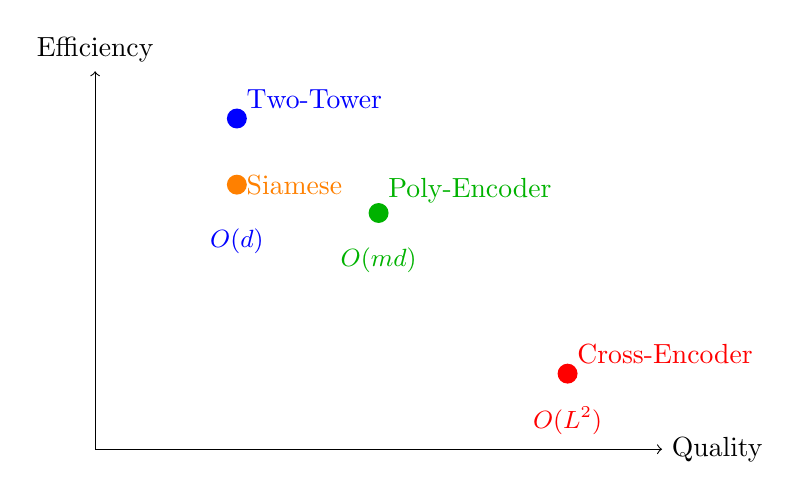
\begin{tikzpicture}[scale=1.2]
    % Axes
    \draw[->] (0,0) -- (6,0) node[right] {Quality};
    \draw[->] (0,0) -- (0,4) node[above] {Efficiency};
    
    % Points
    \fill[blue] (1.5, 3.5) circle (3pt) node[above right] {Two-Tower};
    \fill[orange] (1.5, 2.8) circle (3pt) node[right] {Siamese};
    \fill[green!70!black] (3, 2.5) circle (3pt) node[above right] {Poly-Encoder};
    \fill[red] (5, 0.8) circle (3pt) node[above right] {Cross-Encoder};

    % Annotations (per-candidate scoring cost)
    \node[font=\small, blue] at (1.5, 2.2) {$O(d)$};
    \node[font=\small, green!70!black] at (3, 2) {$O(md)$};
    \node[font=\small, red] at (5, 0.3) {$O(L^2)$};
\end{tikzpicture}
\caption{Trade-off between matching quality and computational efficiency for similarity architectures. Labels give the per-candidate scoring cost once candidate representations are pre-computed: $d$ = embedding dimension, $m$ = number of poly-encoder code vectors, $L$ = joint query--candidate sequence length (the cross-encoder cannot pre-compute anything and pays a full transformer forward pass per pair). Siamese and two-tower are both bi-encoders: they sit in the same quality band, since any quality difference comes from training data and objectives, not the architecture.}
\label{fig:similarity_tradeoff}
\end{figure}

The fundamental trade-off:
\begin{itemize}
    \item \textbf{More interaction} between query and candidate = higher quality
    \item \textbf{Less interaction} = items can be pre-computed = faster retrieval
\end{itemize}

%==============================================================================
\section{Siamese Networks}
\label{sec:siamese}
%==============================================================================

\subsection{Architecture Overview}

Siamese networks process two inputs through identical (weight-shared) encoders and compute similarity in embedding space.

\begin{figure}[H]
\centering
\begin{tikzpicture}[
    node distance=1.5cm,
    box/.style={rectangle, draw, minimum width=2cm, minimum height=0.8cm, rounded corners},
    encoder/.style={box, fill=lightblue},
    input/.style={box, fill=lightgray},
    output/.style={box, fill=lightgreen}
]
    % Inputs
    \node[input] (x1) {Input $x_1$};
    \node[input, right=3cm of x1] (x2) {Input $x_2$};
    
    % Encoders
    \node[encoder, below=1cm of x1] (enc1) {Encoder $f_\theta$};
    \node[encoder, below=1cm of x2] (enc2) {Encoder $f_\theta$};
    
    % Weight sharing indicator
    \draw[<->, thick, dashed, orange] (enc1.east) -- (enc2.west) node[midway, above] {Shared weights};
    
    % Embeddings
    \node[below=1cm of enc1] (z1) {$\vz_1 = f_\theta(x_1)$};
    \node[below=1cm of enc2] (z2) {$\vz_2 = f_\theta(x_2)$};
    
    % Similarity computation
    \node[output, below=1.5cm of $(z1)!0.5!(z2)$] (sim) {$d(\vz_1, \vz_2)$ or $\cos(\vz_1, \vz_2)$};
    
    % Loss
    \node[below=0.8cm of sim] (loss) {Contrastive / Triplet Loss};
    
    % Edges
    \draw[->] (x1) -- (enc1);
    \draw[->] (x2) -- (enc2);
    \draw[->] (enc1) -- (z1);
    \draw[->] (enc2) -- (z2);
    \draw[->] (z1) -- (sim);
    \draw[->] (z2) -- (sim);
    \draw[->] (sim) -- (loss);
\end{tikzpicture}
\caption{Siamese network architecture with shared encoder weights.}
\label{fig:siamese_arch}
\end{figure}

\subsection{Mathematical Formulation}

Let $f_\theta: \mathcal{X} \to \R^d$ be the shared encoder with parameters $\theta$.

For inputs $x_1, x_2$:
\begin{align}
\vz_1 &= f_\theta(x_1) \\
\vz_2 &= f_\theta(x_2) \\
\text{similarity} &= g(\vz_1, \vz_2)
\end{align}

Common similarity functions:
\begin{align}
\text{Cosine:} \quad g(\vz_1, \vz_2) &= \frac{\vz_1^T \vz_2}{\|\vz_1\| \|\vz_2\|} \\
\text{Euclidean:} \quad g(\vz_1, \vz_2) &= -\|\vz_1 - \vz_2\|_2 \\
\text{Learned:} \quad g(\vz_1, \vz_2) &= \text{MLP}([\vz_1; \vz_2; |\vz_1 - \vz_2|; \vz_1 \odot \vz_2])
\end{align}

\subsection{Why Weight Sharing?}

\textbf{Embedding Space Consistency.} Weight sharing ensures inputs of the same type are mapped to a consistent embedding space, enabling meaningful distance comparisons.

Without weight sharing:
\begin{itemize}
    \item Two encoders could learn completely different representations
    \item Distance in ``combined'' space would be meaningless
    \item Need paired training data for both encoders
\end{itemize}

With weight sharing:
\begin{itemize}
    \item Single, consistent embedding space
    \item Any two items can be compared
    \item More parameter-efficient
    \item Acts as regularization
\end{itemize}

\subsection{Training Siamese Networks}

\subsubsection{With Contrastive Loss}

For pair $(x_1, x_2)$ with label $y \in \{0, 1\}$ (1 = similar):
\begin{equation}
\loss = y \cdot d(\vz_1, \vz_2)^2 + (1-y) \cdot \max(0, m - d(\vz_1, \vz_2))^2
\end{equation}

\subsubsection{With Binary Cross-Entropy}

Transform distance to probability:
\begin{equation}
p = \sigma(-\alpha \cdot d(\vz_1, \vz_2) + \beta)
\end{equation}
Then use standard BCE loss.

\subsubsection{Pair Sampling Strategies}

\begin{table}[H]
\centering
\caption{Pair sampling strategies for Siamese networks}
\begin{tabularx}{\textwidth}{lXX}
\toprule
\textbf{Strategy} & \textbf{Description} & \textbf{Trade-off} \\
\midrule
Random & Random positive and negative pairs & Many easy negatives, slow learning \\
Hard negative mining & Find most similar negative pairs & Can cause training instability \\
Semi-hard mining & Negatives within margin of positives & Good balance \\
Online mining & Mine within each batch & Efficient, commonly used \\
Curriculum & Start easy, increase difficulty & Can improve convergence \\
\bottomrule
\end{tabularx}
\end{table}

\subsection{Applications}

\subsubsection{Face Verification}

\begin{itemize}
    \item \textbf{Task}: Given two face images, determine if same person
    \item \textbf{Architecture}: CNN encoder (ResNet, etc.)
    \item \textbf{Training}: Pairs of same/different person images
    \item \textbf{Inference}: Compute embedding distance, threshold
\end{itemize}

\subsubsection{Signature Verification}

\begin{itemize}
    \item \textbf{Task}: Verify if signature matches reference
    \item \textbf{Challenge}: Few examples per person, many forgery types
    \item \textbf{Advantage}: Siamese can work with single reference example
\end{itemize}

\subsubsection{One-Shot Learning}

\begin{itemize}
    \item \textbf{Task}: Classify with one example per class
    \item \textbf{Method}: Compare query to each class example
    \item \textbf{Prediction}: Class with highest similarity
\end{itemize}

\begin{keyinsight}
Siamese networks excel when:
\begin{enumerate}
    \item You need to compare items of the \textbf{same type}
    \item You have \textbf{limited examples} per class (few-shot)
    \item The comparison is \textbf{symmetric} (order doesn't matter)
    \item You need \textbf{interpretable} similarity scores
\end{enumerate}
\end{keyinsight}

%==============================================================================
\section{Triplet Networks}
\label{sec:triplet}
%==============================================================================

\subsection{Architecture Overview}

Triplet networks extend Siamese networks to process three inputs: anchor, positive, and negative.

\begin{figure}[H]
\centering
\begin{tikzpicture}[
    node distance=1cm,
    box/.style={rectangle, draw, minimum width=1.8cm, minimum height=0.7cm, rounded corners},
    encoder/.style={box, fill=lightblue},
    input/.style={box, fill=lightgray, minimum width=1.5cm}
]
    % Inputs
    \node[input] (a) {Anchor};
    \node[input, right=1.5cm of a] (p) {Positive};
    \node[input, right=1.5cm of p] (n) {Negative};
    
    % Encoders
    \node[encoder, below=0.8cm of a] (ea) {$f_\theta$};
    \node[encoder, below=0.8cm of p] (ep) {$f_\theta$};
    \node[encoder, below=0.8cm of n] (en) {$f_\theta$};
    
    % Embeddings
    \node[below=0.8cm of ea] (za) {$\vz_a$};
    \node[below=0.8cm of ep] (zp) {$\vz_p$};
    \node[below=0.8cm of en] (zn) {$\vz_n$};
    
    % Distances
    \node[below=1.2cm of $(za)!0.5!(zp)$, fill=lightgreen, draw, rounded corners] (dp) {$d_+ = d(\vz_a, \vz_p)$};
    \node[below=1.2cm of $(za)!0.5!(zn)$, fill=red!20, draw, rounded corners] (dn) {$d_- = d(\vz_a, \vz_n)$};
    
    % Loss
    \node[below=1cm of $(dp)!0.5!(dn)$] (loss) {$\loss = \max(0, d_+ - d_- + m)$};
    
    % Edges
    \draw[->] (a) -- (ea);
    \draw[->] (p) -- (ep);
    \draw[->] (n) -- (en);
    \draw[->] (ea) -- (za);
    \draw[->] (ep) -- (zp);
    \draw[->] (en) -- (zn);
    \draw[->] (za) -- (dp);
    \draw[->] (zp) -- (dp);
    \draw[->] (za) -- (dn);
    \draw[->] (zn) -- (dn);
    \draw[->] (dp) -- (loss);
    \draw[->] (dn) -- (loss);
    
    % Shared weights
    \draw[<->, dashed, orange] (ea.north) to[bend left=30] (ep.north);
    \draw[<->, dashed, orange] (ep.north) to[bend left=30] (en.north);
\end{tikzpicture}
\caption{Triplet network architecture with shared encoder.}
\label{fig:triplet_arch}
\end{figure}

\subsection{Triplet Loss Analysis}

\begin{mathresult}{Triplet Loss}
\begin{equation}
\loss = \max(0, d(\vz_a, \vz_p) - d(\vz_a, \vz_n) + m)
\end{equation}
where $m > 0$ is the margin.
\end{mathresult}

\subsubsection{Gradient Analysis}

When the loss is active (i.e., $d_+ - d_- + m > 0$):
\begin{align}
\frac{\partial \loss}{\partial \vz_a} &= \frac{\partial d_+}{\partial \vz_a} - \frac{\partial d_-}{\partial \vz_a} \\
\frac{\partial \loss}{\partial \vz_p} &= \frac{\partial d_+}{\partial \vz_p} \\
\frac{\partial \loss}{\partial \vz_n} &= -\frac{\partial d_-}{\partial \vz_n}
\end{align}

For Euclidean distance:
\begin{align}
\frac{\partial \loss}{\partial \vz_a} &\propto (\vz_a - \vz_p) - (\vz_a - \vz_n) = \vz_n - \vz_p \\
\frac{\partial \loss}{\partial \vz_p} &\propto \vz_p - \vz_a \quad \text{(move toward anchor)} \\
\frac{\partial \loss}{\partial \vz_n} &\propto \vz_a - \vz_n \quad \text{(move away from anchor)}
\end{align}

\subsection{Triplet Mining: The Critical Component}

\textbf{Triplet Types.} Given anchor $a$ with positive $p$ and negative $n$:
\begin{itemize}
    \item \textbf{Easy}: $d(a,n) > d(a,p) + m$ — Already satisfied, zero loss
    \item \textbf{Semi-hard}: $d(a,p) < d(a,n) < d(a,p) + m$ — Negative farther but within margin
    \item \textbf{Hard}: $d(a,n) < d(a,p)$ — Negative closer than positive!
\end{itemize}

\begin{figure}[H]
\centering
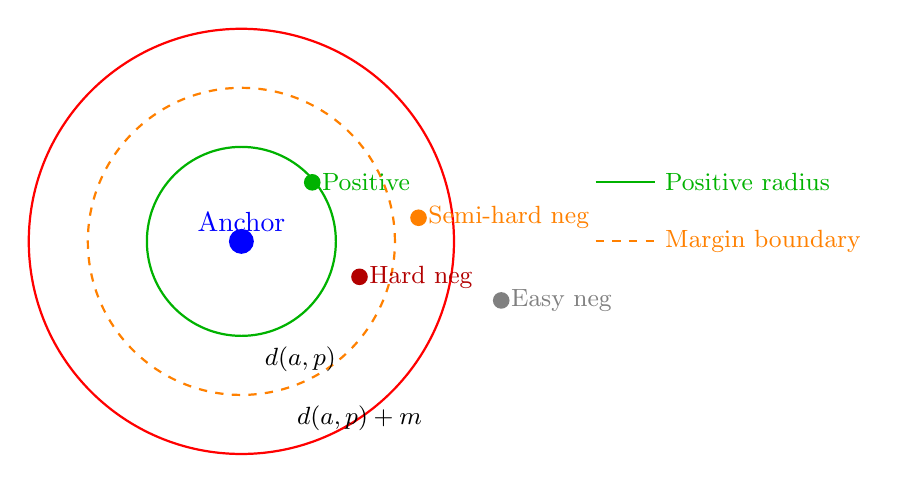
\begin{tikzpicture}[scale=1.5]
    % Anchor
    \fill[blue] (0,0) circle (3pt) node[above] {Anchor};
    
    % Circles
    \draw[green!70!black, thick] (0,0) circle (0.8);
    \draw[orange, thick, dashed] (0,0) circle (1.3);
    \draw[red, thick] (0,0) circle (1.8);
    
    % Points
    \fill[green!70!black] (0.6, 0.5) circle (2pt) node[right, font=\small] {Positive};
    \fill[red!70!black] (1.0, -0.3) circle (2pt) node[right, font=\small] {Hard neg};
    \fill[orange] (1.5, 0.2) circle (2pt) node[right, font=\small] {Semi-hard neg};
    \fill[gray] (2.2, -0.5) circle (2pt) node[right, font=\small] {Easy neg};
    
    % Labels
    \node[font=\small] at (0.5, -1.0) {$d(a,p)$};
    \node[font=\small] at (1.0, -1.5) {$d(a,p)+m$};
    
    % Legend
    \draw[green!70!black, thick] (3, 0.5) -- (3.5, 0.5) node[right, font=\small] {Positive radius};
    \draw[orange, thick, dashed] (3, 0) -- (3.5, 0) node[right, font=\small] {Margin boundary};
\end{tikzpicture}
\caption{Visualization of triplet types based on negative distance from anchor.}
\label{fig:triplet_types}
\end{figure}

\subsubsection{Mining Strategies}

\begin{enumerate}
    \item \textbf{Batch All}: Use all valid triplets in batch
    \begin{itemize}
        \item Pro: No selection bias
        \item Con: Most triplets are easy, wasted computation
    \end{itemize}
    
    \item \textbf{Batch Hard}: For each anchor, hardest positive and hardest negative in batch
    \begin{itemize}
        \item Pro: Maximum learning signal
        \item Con: Can collapse (mislabeled data, outliers)
    \end{itemize}
    
    \item \textbf{Batch Semi-Hard}: Hardest negative that is still farther than positive
    \begin{itemize}
        \item Pro: Informative but not destabilizing
        \item Con: May not exist in small batches
    \end{itemize}
    
    \item \textbf{Distance-Weighted Sampling}: Sample negatives with probability proportional to similarity
    \begin{itemize}
        \item Pro: Smooth curriculum
        \item Con: More complex implementation
    \end{itemize}
\end{enumerate}

\begin{algorithm}[H]
\caption{Batch Semi-Hard Mining}
\begin{algorithmic}[1]
\REQUIRE Embeddings $\{z_i\}$, labels $\{y_i\}$, margin $m$
\STATE Compute pairwise distances $D_{ij} = d(z_i, z_j)$
\FOR{each anchor $a$}
    \STATE $\mathcal{P} \gets \{i : y_i = y_a, i \neq a\}$ \COMMENT{Positives}
    \STATE $\mathcal{N} \gets \{i : y_i \neq y_a\}$ \COMMENT{Negatives}
    \STATE $p^* \gets \argmax_{p \in \mathcal{P}} D_{ap}$ \COMMENT{Hardest positive}
    \STATE $\mathcal{N}_{sh} \gets \{n \in \mathcal{N} : D_{ap^*} < D_{an} < D_{ap^*} + m\}$ \COMMENT{Semi-hard}
    \IF{$\mathcal{N}_{sh} \neq \emptyset$}
        \STATE $n^* \gets \argmin_{n \in \mathcal{N}_{sh}} D_{an}$ \COMMENT{Hardest semi-hard}
        \STATE Add triplet $(a, p^*, n^*)$ to batch
    \ENDIF
\ENDFOR
\RETURN Valid triplets
\end{algorithmic}
\end{algorithm}

\begin{warningbox}
\textbf{Common Pitfall: Embedding Collapse}

With aggressive hard negative mining, embeddings can collapse to a point or subspace. Signs:
\begin{itemize}
    \item All embeddings become very similar
    \item Training loss stays high but validation metrics don't improve
    \item Embedding norms become very small or very large
\end{itemize}

\textbf{Solutions}: Use semi-hard mining, normalize embeddings, add regularization, use larger batches.
\end{warningbox}

\subsection{Margin Selection}

The margin $m$ determines the required separation:

\begin{table}[H]
\centering
\caption{Effect of margin size}
\begin{tabularx}{\textwidth}{lXX}
\toprule
\textbf{Margin} & \textbf{Effect} & \textbf{When to Use} \\
\midrule
Small (0.1-0.3) & Easy to satisfy, classes can be close & Fine-grained similarity \\
Medium (0.3-0.7) & Moderate separation & General retrieval \\
Large (0.7-1.0+) & Strong separation required & Coarse categories \\
\bottomrule
\end{tabularx}
\end{table}

For normalized embeddings ($\|\vz\| = 1$), typical margins: $m \in [0.2, 0.5]$ for Euclidean, $m \in [0.1, 0.3]$ for cosine.

\subsection{Advantages Over Siamese + Contrastive}

\begin{enumerate}
    \item \textbf{Relative ranking}: Only cares about ordering, not absolute distances
    \item \textbf{More informative}: Each triplet provides ranking information
    \item \textbf{Natural for retrieval}: Directly optimizes retrieval objective
\end{enumerate}

%==============================================================================
\section{Two-Tower (Dual Encoder) Architecture}
\label{sec:two_tower}
%==============================================================================

\subsection{Architecture Overview}

Two-tower architecture uses \textit{separate} encoders for queries and items, enabling efficient large-scale retrieval.

\begin{figure}[H]
\centering
\begin{tikzpicture}[
    node distance=1.2cm,
    box/.style={rectangle, draw, minimum width=2.5cm, minimum height=0.8cm, rounded corners},
    tower/.style={box, fill=lightblue, minimum height=2cm, align=center},
    input/.style={box, fill=lightgray},
    output/.style={box, fill=lightgreen}
]
    % Query tower
    \node[input] (q) {Query $q$};
    \node[tower, below=0.8cm of q] (qenc) {Query\\Encoder\\$f_q(\cdot; \theta_q)$};
    \node[below=0.8cm of qenc] (qemb) {$\vq = f_q(q)$};
    
    % Item tower
    \node[input, right=4cm of q] (i) {Item $i$};
    \node[tower, below=0.8cm of i] (ienc) {Item\\Encoder\\$f_i(\cdot; \theta_i)$};
    \node[below=0.8cm of ienc] (iemb) {$\vk = f_i(i)$};
    
    % Similarity
    \node[output, below=1.5cm of $(qemb)!0.5!(iemb)$] (score) {$\text{score} = \vq^T \vk$};
    
    % Edges
    \draw[->] (q) -- (qenc);
    \draw[->] (i) -- (ienc);
    \draw[->] (qenc) -- (qemb);
    \draw[->] (ienc) -- (iemb);
    \draw[->] (qemb) -- (score);
    \draw[->] (iemb) -- (score);
    
    % Note about separate encoders
    \node[font=\small\itshape, text width=3cm, align=center] at ($(qenc)!0.5!(ienc)$) {May share weights\\or be independent};
\end{tikzpicture}
\caption{Two-tower architecture with separate query and item encoders.}
\label{fig:two_tower}
\end{figure}

\subsection{Mathematical Formulation}

Let $f_q: \mathcal{Q} \to \R^d$ be the query encoder and $f_i: \mathcal{I} \to \R^d$ be the item encoder.

\begin{equation}
\text{score}(q, i) = f_q(q)^T f_i(i) = \vq^T \vk
\end{equation}

For retrieval from a corpus $\mathcal{C}$:
\begin{equation}
i^* = \argmax_{i \in \mathcal{C}} \vq^T \vk_i
\end{equation}

\subsection{Key Insight: Decomposability}

The score decomposes into independent query and item computations:

\textbf{Computational Decomposition.} For a query $q$ and $N$ items $\{i_1, \ldots, i_N\}$:
\begin{itemize}
    \item \textbf{Item embeddings}: Can be pre-computed offline, $O(N)$ total
    \item \textbf{Query embedding}: Computed at query time, $O(1)$
    \item \textbf{Scoring}: Dot products, $O(N \cdot d)$ but parallelizable
    \item \textbf{With ANN index}: $O(\log N)$ or $O(1)$ per query
\end{itemize}

This is the fundamental reason two-tower scales to billions of items.

\subsection{Training Two-Tower Models}

\subsubsection{Loss Functions}

\textbf{InfoNCE / Softmax Cross-Entropy:}
\begin{equation}
\loss = -\log \frac{\exp(\vq^T \vk^+ / \tau)}{\exp(\vq^T \vk^+ / \tau) + \sum_{j=1}^{K} \exp(\vq^T \vk_j^- / \tau)}
\end{equation}

\textbf{Batch Softmax (in-batch negatives):}
For batch of $B$ query-item pairs $(q_i, i_i)$:
\begin{equation}
\loss_i = -\log \frac{\exp(\vq_i^T \vk_i / \tau)}{\sum_{j=1}^{B} \exp(\vq_i^T \vk_j / \tau)}
\end{equation}

\subsubsection{Negative Sampling Strategies}

\begin{table}[H]
\centering
\caption{Negative sampling strategies for two-tower training}
\begin{tabularx}{\textwidth}{lXX}
\toprule
\textbf{Strategy} & \textbf{Description} & \textbf{Trade-off} \\
\midrule
In-batch & Other items in batch & Efficient but biased by batch composition \\
Random & Uniformly sampled items & Easy negatives, slow learning \\
Popularity-based & Sample proportional to popularity & Corrects for exposure bias \\
Hard (BM25) & Lexically similar but irrelevant & Better gradients for semantic distinction \\
Hard (model) & High-scoring negatives from current model & Best but expensive, need periodic refresh \\
Mixed & Combine multiple strategies & Often best in practice \\
\bottomrule
\end{tabularx}
\end{table}

\begin{algorithm}[H]
\caption{Two-Tower Training with Mixed Negatives}
\begin{algorithmic}[1]
\REQUIRE Dataset $\mathcal{D}$, query encoder $f_q$, item encoder $f_i$, negative ratio $k$
\FOR{each batch $\mathcal{B} = \{(q_i, i_i^+)\}$}
    \STATE Compute query embeddings: $\vq_i = f_q(q_i)$
    \STATE Compute positive item embeddings: $\vk_i^+ = f_i(i_i^+)$
    \STATE \COMMENT{In-batch negatives}
    \STATE $\mathcal{N}_{ib} = \{(q_i, i_j^+) : j \neq i\}$
    \STATE \COMMENT{Additional hard negatives}
    \FOR{each $q_i$}
        \STATE Sample $k$ hard negatives $\{i_{i1}^-, \ldots, i_{ik}^-\}$
        \STATE Compute: $\vk_{ij}^- = f_i(i_{ij}^-)$
    \ENDFOR
    \STATE Compute loss with all negatives
    \STATE Update $\theta_q, \theta_i$
\ENDFOR
\end{algorithmic}
\end{algorithm}

\subsection{When to Share Weights}

\begin{table}[H]
\centering
\caption{Weight sharing in two-tower models}
\begin{tabularx}{\textwidth}{lXX}
\toprule
\textbf{Scenario} & \textbf{Recommendation} & \textbf{Reason} \\
\midrule
Same modality (text-text) & Share or separate & Sharing: regularization; Separate: more capacity \\
Different modality (text-image) & Separate & Different input structures \\
Asymmetric task & Separate & Query and item have different roles \\
Limited data & Share & Regularization, parameter efficiency \\
\bottomrule
\end{tabularx}
\end{table}

\subsection{Limitations of Two-Tower}

\begin{enumerate}
    \item \textbf{No query-item interaction}: Embeddings computed independently
    \item \textbf{Bottleneck}: All information compressed to fixed-size vector
    \item \textbf{Hard to capture fine-grained matching}: Word-level alignment lost
    \item \textbf{Asymmetric information}: Short queries vs. long documents
\end{enumerate}

%==============================================================================
\section{Cross-Encoder Architecture}
\label{sec:cross_encoder}
%==============================================================================

\subsection{Architecture Overview}

Cross-encoder processes query and item \textit{jointly}, enabling full interaction.

\begin{figure}[H]
\centering
\begin{tikzpicture}[
    node distance=1cm,
    box/.style={rectangle, draw, minimum width=3cm, minimum height=0.8cm, rounded corners},
    encoder/.style={box, fill=lightblue, minimum height=1.5cm, minimum width=4cm, align=center},
    input/.style={box, fill=lightgray},
    output/.style={box, fill=lightgreen}
]
    % Input
    \node[input, minimum width=5cm] (input) {{[CLS]} Query {[SEP]} Item {[SEP]}};
    
    % Encoder
    \node[encoder, below=1cm of input] (enc) {Transformer Encoder\\(BERT, RoBERTa, etc.)};
    
    % CLS output
    \node[below=1cm of enc] (cls) {$\vh_{{[CLS]}}$};
    
    % Score
    \node[output, below=0.8cm of cls] (score) {$\text{score} = \mW^T \vh_{{[CLS]}} + b$};
    
    % Edges
    \draw[->] (input) -- (enc);
    \draw[->] (enc) -- (cls);
    \draw[->] (cls) -- (score);
    
    % Attention visualization
    \node[right=2cm of enc, text width=3cm, font=\small\itshape, align=left] {Full self-attention:\\Query tokens attend\\to Item tokens};
\end{tikzpicture}
\caption{Cross-encoder architecture with joint query-item encoding.}
\label{fig:cross_encoder}
\end{figure}

\subsection{Mathematical Formulation}

Concatenate query and item tokens:
\begin{equation}
\vx = [\text{[CLS]}; q_1; \ldots; q_n; \text{[SEP]}; i_1; \ldots; i_m; \text{[SEP]}]
\end{equation}

Pass through transformer:
\begin{equation}
\mH = \text{Transformer}(\vx)
\end{equation}

Score from [CLS] representation:
\begin{equation}
\text{score}(q, i) = \mW^T \vh_{[CLS]} + b
\end{equation}

\subsection{Why Cross-Encoder is More Accurate}

\begin{enumerate}
    \item \textbf{Full attention}: Every query token attends to every item token
    \item \textbf{Token-level alignment}: Can capture word-level matching
    \item \textbf{Contextualized interaction}: Query meaning influenced by item
    \item \textbf{No information bottleneck}: Not compressed to single vector
\end{enumerate}

\begin{example}[Cross-Encoder Advantage]
Query: ``apple stock price''\\
Item 1: ``Apple Inc. (AAPL) shares rose 3\% today...'' \checkmark\\
Item 2: ``The price of apples at grocery stores...'' $\times$

A two-tower model might struggle because ``apple'' and ``price'' appear in both. Cross-encoder can attend from ``stock'' to ``Inc.'', ``AAPL'', ``shares'' to disambiguate.
\end{example}

\subsection{Computational Cost}

\textbf{Cross-Encoder Complexity.} For query length $n$, item length $m$, and $N$ items:
\begin{itemize}
    \item \textbf{Per pair}: $O((n+m)^2)$ for attention
    \item \textbf{Total for $N$ items}: $O(N \cdot (n+m)^2)$
    \item \textbf{No pre-computation}: Must run for every query-item pair
\end{itemize}

For 1 million items with a 12-layer BERT:
\begin{itemize}
    \item Two-tower: a few milliseconds per query (ANN lookup over pre-computed embeddings; see the QPS estimation question in Section~\ref{sec:similarity_questions})
    \item Cross-encoder: minutes per query on a GPU---batched BERT-base at sequence length 256 sustains $\sim$2--3K pairs/s on an A100 (same estimate), so 1M forward passes take $\sim$5--8 minutes; on CPU it is hours. Either way, orders of magnitude outside any online latency budget.
\end{itemize}

\subsection{When to Use Cross-Encoder}

\begin{itemize}
    \item \textbf{Reranking stage}: Top-k results from fast retrieval
    \item \textbf{Small candidate sets}: $< 1000$ items
    \item \textbf{High-stakes decisions}: When accuracy matters more than speed
    \item \textbf{Fine-grained matching}: Semantic similarity, NLI, QA
\end{itemize}

%==============================================================================
\section{Poly-Encoder and the Architecture Comparison}
\label{sec:poly_encoder}
%==============================================================================

The poly-encoder is the historical middle ground between the two extremes above, and it is worth knowing as the argument that interaction and pre-computation are a dial rather than a binary. The item is encoded to a single vector offline, exactly as in a bi-encoder, but the query is summarized into $m$ learned ``code'' vectors: each $\vy_i^q$ is an attention-weighted pooling of the query token states under a learned code $\vc_i$. The item vector $\vk$ then attends over those codes before scoring:
\begin{equation}
\text{score}(q, i) = \vk^\top \sum_i \text{softmax}\!\left(\vk^\top \vy_i^q\right) \vy_i^q .
\end{equation}
Item embeddings stay pre-computable, so the index is unchanged; scoring costs $O(md)$ per candidate instead of the bi-encoder's $O(d)$, with $m$ typically 16--360, and buys a limited amount of query--item interaction without paying the cross-encoder's $O(L^2)$ per pair.

In current practice the poly-encoder has largely been superseded by \textit{late interaction} (ColBERT and its descendants), which keeps a vector per \textit{token} rather than $m$ learned codes and scores by MaxSim---more expressive, and with a serving story the poly-encoder never got. The late-interaction line, its storage math, and when it earns its cost are [SR 4].

\begin{table}[H]
\centering
\caption{Similarity architectures: what each buys, and what it costs per candidate}
\label{fig:poly_encoder}% label retained; the poly-encoder schematic is folded into this table
\begin{tabularx}{\textwidth}{lXXX}
\toprule
\textbf{Aspect} & \textbf{Bi-encoder (two-tower)} & \textbf{Poly-encoder / late interaction} & \textbf{Cross-encoder} \\
\midrule
Item pre-compute & Yes (one vector) & Yes ($m$ codes, or one vector per token) & No \\
Query--item interaction & None (dot product) & Limited (attention over codes/tokens) & Full self-attention \\
Scoring cost per candidate & $O(d)$ & $O(md)$ & $O(L^2)$ \\
Quality (typical) & Good & Better & Best \\
Practical corpus scale & Billions & Millions & Thousands \\
Funnel position & Retrieval & Retrieval or mid-funnel & Reranking \\
\bottomrule
\end{tabularx}
\end{table}

%==============================================================================
\section{From Architectures to a Funnel}
\label{sec:two_stage}
%==============================================================================

The architectures above are not alternatives; production systems compose them. Because per-candidate cost and per-candidate quality move together, the only way to afford the expensive model is to run it on few candidates---so each stage spends more compute on fewer items than the stage before it. The canonical shape narrows $10^9$ items to $\sim$1000 with a bi-encoder over an ANN index (tens of milliseconds, tuned for \textit{recall}), then to $\sim$100 with a cross-encoder rerank (tuned for \textit{precision at the top}), then to a page with business logic (diversity, freshness, policy).
\label{fig:two_stage}% label retained; the funnel diagram is canon in [SR 4]

Two consequences are worth carrying into any interview. First, the \textbf{recall ceiling}: a candidate the first stage misses cannot be recovered downstream, so the retrieval stage is evaluated on recall@$k$ at its handoff depth, never on precision---and the most common funnel misdiagnosis is tuning the reranker when the candidate set never contained the answer. Second, the cross-encoder sits \textit{last} for an arithmetic reason rather than a stylistic one: it cannot pre-compute anything, so its cost is linear in candidates scored, and a full BERT-base pass over even $10^3$ candidates already blows a typical online budget.

\begin{keyinsight}[Where the Funnel Is Canon]
The funnel as a design object---stage-by-stage candidate counts, a worked latency budget, hybrid lexical/dense fusion, late interaction, LLM rerankers and their economics, and how handoff depths are actually chosen from marginal recall curves---is Volume III, [SR 4]. Index internals and sizing are [SR 3]; caching, freshness, and serving are [SR 8]. This chapter stops where the question stops being ``how were these embeddings trained?''
\end{keyinsight}

%==============================================================================
\section{Approximate Nearest Neighbor Search, in Brief}
\label{sec:ann}
%==============================================================================

A trained item tower is only useful if its output can be searched quickly. Exact search costs $O(Nd)$ per query---at $N = 10^8$ and $d = 768$ that is hundreds of gigabytes of memory traffic per query---so serving uses an \textit{approximate} index that trades a few points of recall for two to three orders of magnitude in speed. The consequence that matters on the training side: brute-force recall measured offline is only an \textit{upper bound} on what the served system delivers, so ANN recall@$k$ has to be monitored as a quantity separate from model quality. A model improvement hidden behind an index regression is indistinguishable from a model regression.

\begin{table}[H]
\centering
\caption{ANN index families at a glance (768-d embeddings; the one-line version)}
\label{fig:hnsw}% label retained; the HNSW layer diagram and its mechanics are canon in [SR 3]
\begin{tabularx}{\textwidth}{lXX}
\toprule
\textbf{Index} & \textbf{Mechanism} & \textbf{Reach for it when} \\
\midrule
Flat (exact) & Full SIMD/GPU scan; recall $=1$ & The corpus is small ($\lesssim$ a few million), or exactness and constant churn matter more than latency \\
HNSW & Hierarchical proximity graph; greedy descent from sparse upper layers to a dense base layer & You want the best recall--QPS trade and can afford vectors $+$ graph resident in RAM \\
IVF-PQ & $k$-means cells plus product-quantized codes; scan only \texttt{nprobe} cells & Memory or cost is the binding constraint; pair with an exact rerank to recover the recall quantization gives up \\
DiskANN & Graph on NVMe with quantized codes in RAM & The corpus is far larger than one node's RAM \\
\bottomrule
\end{tabularx}
\end{table}

The full treatment---why high dimensions break exact indexes, LSH amplification, HNSW graph construction and its $M$/\texttt{ef} parameters, the \texttt{nprobe} recall curve, the quantization ladder from int8 through OPQ and anisotropic PQ, Johnson--Lindenstrauss sketching, and the recall--latency--memory triangle with worked sizing---is Volume III, [SR 3]. Deletes, centroid drift, and reindexing are [SR 8]. What belongs in a training chapter is only the interface: the index searches whatever geometry the loss produced, so a scoring function that disagrees with the index metric---dot-product-trained embeddings served on a cosine index, say---silently costs recall without any error surfacing anywhere. That failure mode is the subject of the cosine-versus-dot-product question below.

%==============================================================================
\section{Architecture Selection Guide}
\label{sec:similarity_arch_selection}
%==============================================================================

This guide is about choosing the architecture you \textit{train}---what the encoders see, and what can be pre-computed. Choosing the serving stack that goes with it (index family, number of stages, latency budget per stage) is [SR 3] and [SR 4].

\begin{figure}[H]
\centering
\begin{tikzpicture}[
    node distance=1cm,
    decision/.style={diamond, draw, aspect=2.5, inner sep=1pt, fill=lightyellow, font=\small},
    result/.style={rectangle, draw, rounded corners, fill=lightgreen, minimum width=2.5cm, font=\small, align=center},
    arrow/.style={->, thick}
]
    % Start
    \node[decision] (scale) {Corpus size?};
    
    % Scale branches
    \node[decision, below left=1.5cm and 1cm of scale] (small) {Latency?};
    \node[decision, below right=1.5cm and 1cm of scale] (large) {Real-time?};
    
    % Results
    \node[result, below left=1cm and 0cm of small] (cross) {Cross-Encoder};
    \node[result, below right=1cm and 0cm of small] (poly) {Poly-Encoder /\\Late Interaction};
    \node[result, below left=1cm and 0cm of large] (twostage) {Two-Stage\\(Two-Tower + Rerank)};
    \node[result, below right=1cm and 0cm of large] (tower) {Two-Tower Only};
    
    % Edges
    \draw[arrow] (scale) -- node[above left, font=\small] {$<$10K} (small);
    \draw[arrow] (scale) -- node[above right, font=\small] {$>$10K} (large);
    \draw[arrow] (small) -- node[left, font=\small] {Flexible} (cross);
    \draw[arrow] (small) -- node[right, font=\small] {$<$100ms} (poly);
    \draw[arrow] (large) -- node[left, font=\small] {Yes} (twostage);
    \draw[arrow] (large) -- node[right, font=\small] {Batch} (tower);
\end{tikzpicture}
\caption{Decision tree for similarity architecture selection.}
\label{fig:arch_decision}
\end{figure}

\begin{table}[H]
\centering
\caption{Architecture selection by use case}
\begin{tabularx}{\textwidth}{lXX}
\toprule
\textbf{Use Case} & \textbf{Recommended} & \textbf{Notes} \\
\midrule
Face verification & Siamese & Same image type, symmetric \\
Image search (1M+) & Two-Tower + HNSW & Pre-compute image embeddings \\
Document retrieval (1B) & Two-Stage & Two-tower retrieval + cross-encoder rerank \\
Semantic similarity & Cross-Encoder & Full interaction needed \\
Recommendation & Two-Tower & User/item can be pre-computed \\
QA retrieval & Two-Stage & Dense retrieval + reader \\
Duplicate detection & Siamese or Two-Tower & Depends on scale \\
Few-shot classification & Siamese & Compare to class examples \\
\bottomrule
\end{tabularx}
\end{table}

%==============================================================================
\section{Interview Questions}
\label{sec:similarity_questions}
%==============================================================================

\begin{keyinsight}[Questions That Moved to Volume III]
Three questions this chapter used to carry are canon elsewhere now, because they are systems questions rather than training questions. \textbf{``Design a multi-stage retrieval pipeline''}---the one canonical retrieval-design answer, with per-stage candidate counts and a worked latency budget---is [SR 4]. \textbf{``Estimate the ANN index size and query latency for 1B 768-dim embeddings''} is [SR 3], which works the sizing arithmetic for flat, HNSW, IVF-PQ, and DiskANN side by side. \textbf{``Update embeddings in production without re-indexing''} is [SR 8], alongside blue-green reindexing, why HNSW hates deletes, and what an embedding refresh actually costs. Prepare those there; the questions below are the ones whose answer is about the objective, the negatives, and the geometry.
\end{keyinsight}

%--- Q1 ---

\begin{interviewq}
\textbf{Q: Your two-tower model retrieves documents that share keywords with the query but aren't actually relevant. How do you fix this?}

\badgeLfive{L5} \quad \badgetype{Debugging} \quad \badgefreq{\freqhigh}

\stronganswer

This is a classic failure mode: the two-tower model has learned \textit{lexical matching} instead of \textit{semantic matching}. The dot product of query and document embeddings correlates with keyword overlap rather than relevance. I would diagnose and fix in stages.

\textbf{Diagnosis.} Retrieve the top-50 results for 100 diverse queries. Annotate each result as relevant/irrelevant. For the false positives, check: do they share specific keywords with the query? If so, this confirms the lexical matching hypothesis. Also compute BM25 scores for the same queries---if BM25 and the two-tower model agree on most results, the model has effectively learned BM25 in embedding space.

\textbf{Root cause: insufficient hard negatives.} With random or in-batch negatives, the model only needs to distinguish topically unrelated items (easy) and never learns to distinguish ``keyword-similar but irrelevant'' from ``truly relevant.'' The gradient signal from easy negatives is near zero.

\textbf{Fix 1: BM25 hard negatives.} For each query, retrieve the top-100 BM25 results, filter out the true positives, and use the remaining as hard negatives. These share keywords with the query but were not clicked/labeled as relevant. Training against these specifically teaches the model to go beyond lexical matching. Mix hard negatives with random negatives (e.g., 30\% hard, 70\% random) to avoid training instability from exclusively hard examples.

\textbf{Fix 2: Paraphrase augmentation.} Add paraphrased queries as positives---these have the same meaning but different words. This forces the model to encode meaning rather than specific word patterns. Generate paraphrases using back-translation or an LLM.

\textbf{Fix 3: Add a cross-encoder reranking stage.} Even with improved embeddings, a two-tower model cannot capture fine-grained query-document interactions. A cross-encoder reranker on the top-100 candidates captures word-level alignment and resolves ambiguity (e.g., ``apple stock price'' vs. ``price of apples''). This is the most reliable fix and is standard in production search systems.

\textbf{Fix 4: Pre-train with contrastive objectives.} Start from a model already trained for retrieval (E5, BGE) rather than vanilla BERT. These models have already learned to distinguish semantic from lexical similarity during their pre-training.

\redflags
\begin{itemize}
    \item ``Just increase the model size''---this doesn't fix the training signal problem.
    \item Not mentioning hard negatives---this is the single most impactful fix for this failure mode.
    \item ``Remove keywords from the query''---this destroys information rather than improving the model.
\end{itemize}

\interviewtest{Diagnosis of a specific retrieval failure mode (lexical vs. semantic matching), understanding of why it happens (training signal from easy negatives), and knowledge of the standard fix (hard negatives from BM25).}

\goodgreat
\begin{itemize}
    \item \badgeLfive{L5} Identifies hard negative mining as the key fix, proposes BM25-based negatives.
    \item \badgeLsix{L6} Adds the diagnosis step (confirming the lexical matching hypothesis), proposes a mixed negative strategy, and adds cross-encoder reranking as a complementary fix.
    \item \badgeLseven{L7} Discusses the curriculum of negative difficulty (start with moderate negatives, increase difficulty over training), proposes an asynchronous hard negative mining pipeline that refreshes negatives as the model improves, and notes that the hardest negatives should be mined from the \textit{current} model, not a static BM25 ranker.
\end{itemize}

\followups{``How often should you refresh hard negatives during training?'' ``What happens if you use only hard negatives?'' ``How do you measure whether the model is doing lexical vs. semantic matching?''}
\end{interviewq}

%--- Q2 ---

\begin{interviewq}
\textbf{Q: Siamese vs Triplet vs Two-Tower---decision framework for a new retrieval project.}

\badgeLfive{L5} \quad \badgetype{Trade-off} \quad \badgefreq{\freqhigh}

\stronganswer

These architectures form a spectrum from simple symmetric comparison to scalable asymmetric retrieval. The choice depends on the problem structure.

\textbf{Siamese networks} use a single shared encoder for both inputs. Best when: (1) the two inputs are the same type (image-image, sentence-sentence), (2) comparison is symmetric (order doesn't matter), (3) you have limited training data (weight sharing acts as strong regularization), and (4) the corpus is small enough that pairwise comparison is feasible ($<$100K items). Classic use cases: face verification, signature verification, one-shot learning. Loss: contrastive loss or cosine similarity loss on pairs.

\textbf{Triplet networks} extend Siamese with anchor-positive-negative triplets and triplet loss: $\loss = \max(0, d(a,p) - d(a,n) + m)$. Better than Siamese when: (1) you care about \textit{relative ranking} rather than absolute similarity, (2) you have enough data to construct informative triplets (requires many examples per class for good mining). Key challenge: triplet mining---easy triplets contribute zero gradient, hard triplets can destabilize training. Semi-hard mining is the standard default. Use cases: image retrieval, person re-identification, fine-grained visual similarity.

\textbf{Two-tower (dual encoder)} uses separate encoders for queries and items, enabling asymmetric inputs and pre-computed item embeddings. Choose when: (1) query and item types differ (text query, product item), (2) the corpus is large ($>$1M items)---item embeddings are computed once and indexed, (3) real-time retrieval is needed ($<$10ms), (4) you need to serve high QPS (queries per second). Training typically uses InfoNCE with in-batch negatives + hard negatives. Use cases: search, recommendation, ad matching.

\textbf{Decision framework:}
\begin{itemize}
    \item Same-type symmetric comparison + small corpus $\to$ Siamese
    \item Same-type ranking + medium corpus + abundant per-class data $\to$ Triplet
    \item Cross-type or large-scale retrieval + latency constraints $\to$ Two-tower
    \item Any scale where precision matters more than latency $\to$ Cross-encoder (not covered above, but often used as a reranker on top of two-tower)
\end{itemize}

In practice, modern systems often skip the Siamese/Triplet distinction and go directly to two-tower with InfoNCE loss (which subsumes both contrastive and triplet objectives when using in-batch negatives).

\redflags
\begin{itemize}
    \item ``Triplet networks are outdated''---they remain effective for fine-grained similarity where per-class data is abundant.
    \item ``Two-tower is always better''---for symmetric same-type comparison with limited data, Siamese with weight sharing is more data-efficient.
    \item Not mentioning scale as the primary decision factor.
\end{itemize}

\interviewtest{Ability to choose the right architecture for a given problem by reasoning about the constraints (data type, corpus size, latency, training data availability) rather than always defaulting to the most popular approach.}

\goodgreat
\begin{itemize}
    \item \badgeLfive{L5} Clearly states when each architecture is appropriate, mentions scale as the key differentiator.
    \item \badgeLsix{L6} Discusses how InfoNCE subsumes contrastive and triplet objectives, explains the weight-sharing decision for two-tower, and proposes combining two-tower + cross-encoder for production systems.
    \item \badgeLseven{L7} Discusses evolution from these discrete architecture choices to unified contrastive frameworks (CLIP-style) that scale seamlessly, and how modern systems often blend retrieval architectures (multiple two-tower models + BM25 + cross-encoder) in an ensemble.
\end{itemize}

\followups{``When would you use both a Siamese and a two-tower model in the same system?'' ``How does the loss function choice differ across architectures?'' ``What is the minimum training data needed for each?''}
\end{interviewq}

%--- Q3 ---

\begin{interviewq}
\textbf{Q: Your two-tower model's recall@10 is good but precision@10 is poor. What's wrong?}

\badgeLsix{L6} \quad \badgetype{Debugging} \quad \badgefreq{\freqmed}

\stronganswer

Good recall@10 means the model \textit{can} retrieve relevant documents in the top 10. Poor precision@10 means the top 10 also contains many irrelevant documents. This is a \textit{ranking quality} problem within the retrieved set, not a retrieval failure.

\textbf{Diagnosis 1: Insufficient discrimination among close embeddings.} The two-tower model maps both relevant and semi-relevant documents near the query in embedding space. All 10 retrieved documents are ``close'' to the query, but the model can't distinguish ``highly relevant'' from ``somewhat related.'' This happens when: (a) training used only binary relevance labels (relevant/not) without graded relevance, so the model learns a coarse boundary; (b) the embedding dimension is too low to capture fine-grained distinctions; (c) the InfoNCE temperature is too high, making the loss insensitive to small similarity differences.

\textbf{Diagnosis 2: Popularity bias.} Popular items appear as in-batch negatives less often (or are actually clicked frequently regardless of relevance). The model learns to rank popular items highly even when they're not relevant to the specific query. Check: are the false positives in the top-10 disproportionately popular items?

\textbf{Diagnosis 3: The evaluation reveals a fundamental two-tower limitation.} The two-tower model computes query and document embeddings independently---no cross-attention between them. Fine-grained relevance often requires understanding how specific query terms relate to specific document phrases. The two-tower model compresses the document to a single vector, losing word-level matching information.

\textbf{Fixes:}
\begin{enumerate}
    \item \textbf{Add a cross-encoder reranker}: Rerank the top-10 (or top-100 to give the reranker more candidates) with a cross-encoder. This is the most reliable fix because the cross-encoder provides full query-document interaction.
    \item \textbf{Graded relevance training}: If you have graded labels, use a listwise loss (LambdaLoss) or margin-based loss that preserves the relevance ordering, not just binary in/out.
    \item \textbf{Lower the temperature}: A lower $\tau$ in InfoNCE sharpens the similarity distribution, increasing discrimination among similar items. But too low causes training instability---tune carefully.
    \item \textbf{Hard negative calibration}: Ensure hard negatives are ``hard but irrelevant,'' not ``actually relevant but unlabeled.'' Poor hard negatives can teach the model to push away relevant items.
    \item \textbf{Popularity debiasing}: Apply inverse propensity weighting or a popularity correction in the loss to reduce the model's tendency to rank popular items highly regardless of query relevance.
\end{enumerate}

\redflags
\begin{itemize}
    \item ``Increase recall@K to get better precision''---recall@10 is already good, the problem is ranking within the top 10.
    \item ``Train longer''---this is a structural limitation of two-tower models, not a convergence issue.
    \item Confusing precision@10 with overall precision across the entire corpus.
\end{itemize}

\interviewtest{Understanding the difference between retrieval (finding relevant items at all) and ranking (ordering them correctly), and the fundamental limitation of two-tower models for fine-grained ranking.}

\goodgreat
\begin{itemize}
    \item \badgeLfive{L5} Identifies the ranking-within-retrieved-set problem and proposes a cross-encoder reranker.
    \item \badgeLsix{L6} Adds popularity bias diagnosis, temperature tuning, and graded relevance training. Explains the information bottleneck of single-vector representations.
    \item \badgeLseven{L7} Proposes a Poly-Encoder as a middle ground (richer interaction than two-tower without the full cost of a cross-encoder), discusses late interaction models (ColBERT) that retain token-level matching while enabling pre-computation, and designs a monitoring system that tracks precision@K per query category to detect systematic ranking failures.
\end{itemize}

\followups{``How would you measure ranking quality vs retrieval quality separately?'' ``What is a late-interaction model and how does it help?'' ``How does ColBERT compare to a standard cross-encoder?''}
\end{interviewq}

%--- Q4 ---

\begin{interviewq}
\textbf{Q: Cross-encoder vs bi-encoder---when is the quality gap worth the latency cost?}

\badgeLfive{L5} \quad \badgetype{Trade-off} \quad \badgefreq{\freqhigh}

\stronganswer

A bi-encoder (two-tower) computes query and document embeddings independently, enabling $O(1)$ retrieval with pre-computed document vectors. A cross-encoder processes query and document jointly through full self-attention, providing $O(N)$ inference cost (one forward pass per candidate). The quality gap between them typically ranges from 3--8\% on NDCG@10 for retrieval benchmarks, sometimes more for complex semantic matching tasks.

\textbf{When the quality gap is worth the cost:}

(1) \textbf{Reranking a small candidate set.} When a bi-encoder has already reduced 1B documents to 100--1000 candidates, running a cross-encoder on this small set adds tens of milliseconds of latency ($\sim$35--60ms for 100 candidates with BERT-base on an A100; a 1000-candidate set needs a distilled reranker to stay in that range). The quality improvement is almost always worth it because: you're only paying for $\sim$100--1000 forward passes (not millions), and the reranker directly improves the user-visible top-K results.

(2) \textbf{High-stakes decisions.} In legal document review, medical literature search, or compliance checks, a 5\% improvement in ranking quality can have significant downstream impact. The additional latency (even seconds) is acceptable if the decision quality matters more than response time.

(3) \textbf{Offline batch processing.} For tasks like building a curated dataset, computing document similarity matrices, or generating training labels, latency doesn't matter. Use the cross-encoder for maximum quality.

(4) \textbf{Complex semantic matching.} Tasks where word-level interaction is critical---natural language inference, fact verification, fine-grained relevance---benefit disproportionately from cross-encoder's full attention. The quality gap can be $>$10\% for these tasks.

\textbf{When the latency cost is not worth it:}

(1) \textbf{Real-time retrieval at scale.} If you need $<$10ms latency on 1M+ documents, a cross-encoder is infeasible (even at 100 candidates, 10ms is tight for a cross-encoder). Use a well-tuned bi-encoder, possibly with late-interaction (ColBERT) for a middle ground.

(2) \textbf{High QPS with tight SLAs.} At 10K+ QPS with p99 latency requirements, the GPU cost of running cross-encoders on every request may exceed the quality benefit. A distilled bi-encoder that closes part of the quality gap is often preferable.

(3) \textbf{When the quality gap is small.} On some benchmarks and domains, a well-trained bi-encoder (E5, BGE with hard negatives) approaches cross-encoder quality. Always measure the actual gap on your data before adding the complexity of a reranker.

\textbf{The standard production pattern:} Bi-encoder retrieval (top-100 to top-1000) $\to$ cross-encoder reranking (top-10 to top-100). This gets $\sim$95\% of the cross-encoder's quality at $\sim$1\% of the cost of running it on the full corpus.

\redflags
\begin{itemize}
    \item ``Cross-encoder is always better''---it depends on the domain-specific quality gap and latency constraints.
    \item ``Just use a bigger bi-encoder to close the gap''---the gap is \textit{architectural} (independent vs. joint encoding), not just about model size.
    \item Not quantifying the latency difference---it's a concrete engineering trade-off, not abstract.
\end{itemize}

\interviewtest{Whether you can make nuanced cost-benefit trade-offs in system design, quantify both the quality and latency dimensions, and know the standard production pattern.}

\goodgreat
\begin{itemize}
    \item \badgeLfive{L5} Clearly explains the quality-latency trade-off, knows the standard two-stage pattern.
    \item \badgeLsix{L6} Quantifies the quality gap (3--8\% NDCG), mentions ColBERT as a middle ground, and discusses the economics (GPU cost vs. quality improvement).
    \item \badgeLseven{L7} Discusses how to optimally allocate the latency budget across stages (e.g., investing more in the reranker by reducing the candidate set), proposes distilling the cross-encoder into a better bi-encoder (knowledge distillation from reranker to retriever), and discusses emerging approaches that blur the bi/cross boundary (Poly-Encoder, ColBERTv2, SPLADE).
\end{itemize}

\followups{``How would you distill a cross-encoder into a bi-encoder?'' ``What is ColBERT and how does it compare?'' ``How do you decide the candidate set size for reranking?''}
\end{interviewq}

%--- Q5 ---

\begin{interviewq}
\textbf{Q: Hard negative mining strategies---how to choose and when each fails.}

\badgeLsix{L6} \quad \badgetype{Trade-off} \quad \badgefreq{\freqmed}

\stronganswer

Hard negative mining is the process of selecting training negatives that are challenging for the model---items that are similar to the query but not relevant. The choice of mining strategy significantly impacts model quality and training stability.

\textbf{Strategy 1: In-batch negatives.} Use other items in the same batch as negatives. Effective batch size of negatives = $B - 1$ per query. \textit{Pros}: Zero extra computation, naturally diverse. \textit{Fails when}: Batch size is small (weak negative signal), or when the dataset has selection bias (items in the same batch may be from similar categories, making all negatives too easy). \textit{Fix}: Increase batch size, or use cross-GPU negative sharing (gather negatives from all GPUs).

\textbf{Strategy 2: BM25 hard negatives.} For each query, retrieve top-K BM25 results, remove true positives, use the rest as negatives. These share keywords with the query but are irrelevant. \textit{Pros}: Cheap to compute (BM25 is fast), excellent for teaching lexical-vs-semantic distinction. \textit{Fails when}: The task requires semantic-only matching (BM25 negatives may be too easy for an already semantically-trained model), or when BM25 returns items that are actually relevant but unlabeled (false negatives in your training data).

\textbf{Strategy 3: Model-mined hard negatives.} Use the current model's retrieval results as negatives (top-K retrieved but not labeled as relevant). \textit{Pros}: Most informative---these are exactly the items the model currently confuses. \textit{Fails when}: The model's negatives are so hard that many are actually relevant but unlabeled---this teaches the model to push away good results (catastrophic). Also, the model's view of ``hard'' changes during training, so static mining becomes stale. \textit{Fix}: Re-mine periodically (every 5--10K steps), use a separate ``teacher'' model for mining, or add a relevance filter (dedup against known positives, use an LLM to filter).

\textbf{Strategy 4: Cross-batch memory bank (MoCo-style).} Maintain a queue of recent embeddings as a large pool of negatives. \textit{Pros}: Effectively very large negative set without increasing batch size. \textit{Fails when}: Embeddings in the queue become stale as the model updates (the encoder has changed since those embeddings were computed). \textit{Fix}: Use a momentum-updated encoder for the queue (MoCo), or refresh the queue frequently.

\textbf{Strategy 5: Mixed negatives.} Combine multiple sources: 60\% in-batch, 20\% BM25, 20\% model-mined. \textit{Pros}: Diversity of difficulty levels prevents overfitting to one type of negative. \textit{This is the standard practice} for production retrieval models.

\textbf{General principle:} Negatives should be hard enough to provide gradient signal but not so hard that they're actually positive (false negatives). The optimal difficulty is \textit{semi-hard}: negatives that are close to the decision boundary but on the correct side.

\redflags
\begin{itemize}
    \item ``Always use the hardest negatives possible''---this causes training instability and false negative poisoning.
    \item ``Random negatives are sufficient''---they're too easy for any non-trivial model.
    \item Not mentioning the false negative problem with hard mining.
\end{itemize}

\interviewtest{Deep understanding of how negative sampling affects contrastive learning dynamics, awareness of failure modes for each strategy, and practical knowledge of the standard mixed-negative approach.}

\goodgreat
\begin{itemize}
    \item \badgeLfive{L5} Knows BM25 negatives and in-batch negatives, understands why hard negatives help.
    \item \badgeLsix{L6} Discusses false negative poisoning, staleness of model-mined negatives, and proposes the mixed-negative strategy with specific ratios.
    \item \badgeLseven{L7} Designs an automated hard negative mining pipeline with: periodic re-mining, relevance filtering (LLM-based or human-in-the-loop), difficulty annealing (start with easier negatives, increase difficulty during training), and monitoring for false negative rate in the mined set.
\end{itemize}

\followups{``How do you detect that your hard negatives contain false negatives?'' ``How often should you re-mine?'' ``What is the interaction between negative difficulty and learning rate?''}
\end{interviewq}

%--- Q6 ---

\begin{interviewq}
\textbf{Q: Cosine similarity vs dot product vs L2 distance for embeddings---when each?}

\badgeLfive{L5} \quad \badgetype{Conceptual} \quad \badgefreq{\freqhigh}

\stronganswer

These three metrics are closely related but differ in whether they account for embedding magnitude, which has practical implications.

\textbf{Cosine similarity}: $\cos(\vu, \vv) = \frac{\vu^T\vv}{\|\vu\|\|\vv\|}$. Measures the angle between vectors, ignoring magnitude. Range: $[-1, 1]$. \textbf{Use when:} (1) You want purely directional similarity (semantic similarity regardless of ``confidence'' or frequency). (2) Embeddings have variable norms (e.g., frequent items have larger norms due to more gradient updates). (3) Combining embeddings from different models or scales. \textbf{Practical note:} If you L2-normalize all embeddings to unit norm at indexing time, cosine similarity equals dot product, and you can use the faster dot product at query time.

\textbf{Dot product}: $\vu^T\vv = \|\vu\|\|\vv\|\cos(\vu,\vv)$. Measures both angular similarity and magnitude. Range: $(-\infty, \infty)$. \textbf{Use when:} (1) Magnitude carries useful information---e.g., the norm of a document embedding correlates with document quality or relevance, and you want the retrieval score to reflect this. (2) MIPS (Maximum Inner Product Search) is your retrieval primitive---most ANN libraries are optimized for this. (3) Embeddings are already normalized (then dot product = cosine). \textbf{Example:} In recommendation systems, item embedding norms often correlate with popularity. Dot product naturally boosts popular items, which may be desirable.

\textbf{L2 (Euclidean) distance}: $\|\vu - \vv\|_2 = \sqrt{\sum_i(u_i-v_i)^2}$. Measures geometric distance. Range: $[0, \infty)$. \textbf{Use when:} (1) You need a proper distance metric (triangle inequality holds, useful for clustering algorithms). (2) The embedding space was trained with L2-based losses (triplet loss with Euclidean distance, contrastive loss with distance). (3) You're doing k-means clustering on embeddings. \textbf{Relationship:} For unit-normalized vectors, $\|\vu - \vv\|_2^2 = 2(1 - \cos(\vu,\vv))$, so L2 distance is a monotonic function of cosine similarity. In this case, all three metrics produce the same nearest-neighbor ranking.

\textbf{Key insight for interviews:} The choice matters most when embeddings are \textit{not} normalized. With L2-normalized embeddings, all three metrics produce identical rankings, so the choice is purely about computational convenience (dot product is fastest for ANN search).

\textbf{When the choice has real impact:}
\begin{itemize}
    \item \textit{Unnormalized embeddings}: Dot product favors high-norm vectors (popular/frequent items). Cosine ignores this. L2 penalizes large-norm differences. Choose based on whether popularity bias is desired.
    \item \textit{Multi-modal embeddings}: CLIP normalizes embeddings to the unit sphere, so all metrics are equivalent. But if combining CLIP with other features (price, recency), dot product on unnormalized concatenated vectors lets different feature groups contribute different magnitudes.
    \item \textit{ANN index compatibility}: HNSW natively supports L2 and inner product. Faiss supports all three. Choose based on your infrastructure.
\end{itemize}

\redflags
\begin{itemize}
    \item ``Cosine is always best for embeddings''---it depends on whether magnitude carries useful information.
    \item Not knowing the equivalence for normalized vectors---this is the most commonly tested fact.
    \item ``L2 distance and cosine similarity are unrelated''---they are monotonically related for unit vectors.
\end{itemize}

\interviewtest{Understanding of when these metrics differ (unnormalized embeddings), when they're equivalent (normalized), and practical judgment about which to use in different scenarios.}

\goodgreat
\begin{itemize}
    \item \badgeLfive{L5} Correctly explains all three metrics, knows the equivalence for normalized vectors, and picks appropriate use cases.
    \item \badgeLsix{L6} Discusses the magnitude/popularity bias in dot product, the normalize-then-dot-product trick for efficient ANN search, and the interaction with the loss function used during training.
    \item \badgeLseven{L7} Discusses how the choice of similarity metric at training time must match the metric at inference time (training with cosine loss but retrieval with dot product on unnormalized embeddings will fail), and how to handle the case where you want cosine similarity for ranking but dot product for ANN efficiency.
\end{itemize}

\followups{``How does the choice of similarity metric interact with ANN algorithms?'' ``What is MIPS and why is it the standard retrieval primitive?'' ``How would you handle a case where you want cosine for ranking but dot product for speed?''}
\end{interviewq}

%--- Q7 ---

\begin{interviewq}
\textbf{Q: Your contrastive model produces good embeddings for frequent items but poor for rare items. Why?}

\badgeLseven{L7} \quad \badgetype{Debugging} \quad \badgefreq{\freqlow}

\stronganswer

This is a fundamental challenge in contrastive learning: \textit{frequency bias}. Frequent items appear in many training pairs and receive abundant gradient updates, while rare items appear in few pairs and their embeddings are under-trained. The problem has multiple interacting causes.

\textbf{Cause 1: Gradient imbalance.} In contrastive learning, each item's embedding is updated when it appears as a positive or a hard negative. Frequent items (e.g., popular products, common queries) appear in thousands of training pairs; rare items appear in tens. The cumulative gradient signal for frequent items is orders of magnitude larger, so their embeddings converge to high-quality representations while rare item embeddings remain noisy.

\textbf{Cause 2: In-batch negative bias.} With in-batch negatives, frequent items are more likely to appear in the batch and serve as negatives. The model learns to ``push away'' from frequent items (because it sees them as negatives often), effectively learning to discriminate them well. Rare items rarely appear as negatives, so the model never learns to distinguish them from nearby items.

\textbf{Cause 3: Embedding norm disparity.} Without L2 normalization, frequent items develop larger embedding norms (more gradient updates = larger weights). Dot-product similarity then systematically favors frequent items over rare ones, regardless of semantic relevance. Even with normalization, the \textit{direction} of frequent item embeddings is better calibrated.

\textbf{Cause 4: Hard negative mining ignores rare items.} Model-mined hard negatives are biased toward frequent items (they appear in more retrieval results). Rare items are rarely retrieved and therefore rarely selected as hard negatives, further reducing the training signal for the rare-item region of embedding space.

\textbf{Fixes:}
\begin{enumerate}
    \item \textbf{Inverse frequency sampling}: Up-sample rare items in training pairs so each item appears with roughly equal frequency. Weight the loss by inverse document frequency.
    \item \textbf{Separate embedding heads}: Use a shared backbone but add a projection head specifically trained with a higher weight on rare-item pairs.
    \item \textbf{Temperature annealing by frequency}: Use a lower temperature ($\tau$) for rare-item pairs, creating stronger gradient signal per pair to compensate for fewer pairs.
    \item \textbf{Synthetic augmentation}: Generate synthetic variations of rare items (text paraphrasing, image augmentation) to increase their effective training frequency.
    \item \textbf{Pre-trained initialization}: Initialize the embedding model from a strong pre-trained model (CLIP, E5) that has already seen diverse data. The pre-trained representations provide a better starting point for rare items than random initialization.
    \item \textbf{Nearest-neighbor regularization}: Regularize rare item embeddings toward the centroid of their category's embeddings. This leverages the category-level structure learned from frequent items.
\end{enumerate}

\redflags
\begin{itemize}
    \item ``Just train longer''---more training actually widens the gap (frequent items improve faster).
    \item ``Use a larger model''---the bias is in the training distribution, not model capacity.
    \item Not identifying the frequency imbalance as the root cause.
\end{itemize}

\interviewtest{Understanding of how training data distribution affects learned representations, ability to identify the multiple interacting mechanisms that create frequency bias, and knowledge of mitigation strategies.}

\goodgreat
\begin{itemize}
    \item \badgeLfive{L5} Identifies gradient imbalance as the cause and proposes up-sampling.
    \item \badgeLsix{L6} Adds in-batch negative bias, embedding norm disparity, and temperature annealing. Proposes measuring embedding quality stratified by item frequency to quantify the gap.
    \item \badgeLseven{L7} Connects to the broader long-tail problem in retrieval systems, proposes a curriculum that first trains on all data (building general representations) then fine-tunes with emphasis on rare items (improving the tail), and discusses how this interacts with the ANN index (rare items may be poorly indexed because their embedding neighborhoods are noisy).
\end{itemize}

\followups{``How do you measure embedding quality separately for frequent and rare items?'' ``How does this interact with the ANN index?'' ``What is the cold-start problem for new items and how does it relate?''}
\end{interviewq}

%--- Q8 ---

\begin{interviewq}
\textbf{Q: Estimate the QPS of a retrieval system using HNSW on 100M documents. Then add a cross-encoder reranker over the top 100---what changes?}

\badgeLsix{L6} \quad \badgetype{Estimation} \quad \badgefreq{\freqmed}

\stronganswer

Two stages with two different bottlenecks: retrieval is memory-bound on CPU, reranking is compute-bound on GPU. Estimate them separately, then quote the binding one.

\textbf{Stage 1: HNSW per-query latency.} Search evaluates roughly $ef\_search$ candidates (typically 64--256 for good recall); at $ef\_search = 128$ plus traversal bookkeeping, call it $\sim$256 distance computations. The arithmetic is negligible---$256 \times 768 \times 2 \approx 400$K FLOPs, microseconds on an AVX-512 core. The cost is memory access, and the right unit is a \textit{full vector fetch}, not a single cache miss: each 768-dim FP32 vector is 3\,KB $=$ 48 cache lines, and graph traversal jumps to random neighbors, so those lines mostly come from DRAM at $\sim$100\,ns. That gives $256 \times 48 \times 100\,\mathrm{ns} \approx 1.2$\,ms, clawed back somewhat by hardware prefetching within each contiguous vector and L3 hits on hot graph regions. Call it \textbf{0.5--2\,ms per query per thread}.

\textbf{Memory check, always.} $10^8 \times 768 \times 2$ bytes (FP16) $= 154$\,GB, plus $\sim$96\,B/vector of graph ($M = 16$, 32-bit neighbor IDs) $\approx 10$\,GB, so $\sim$164\,GB fits one 256\,GB machine. Had it not fit, the whole estimate changes shape---sharding, or a compressed index ([SR 3]).

\textbf{Stage-1 QPS.} 32--64 cores at $\sim$1\,ms per query is tens of thousands of QPS in principle; after network, serialization, and load balancing, \textbf{$\sim$10--20K QPS per machine} is the number to quote. Serving 100K QPS is then 5--10 replicas of the full index behind a load balancer: replication buys QPS, sharding buys corpus size. INT8 or scalar quantization shrinks the footprint \textit{and} improves cache hit rate, roughly doubling QPS.

\textbf{Stage 2: cross-encoder over the top 100.} The arithmetic inverts. One BERT-base pass at sequence length 256 is $\sim$56 GFLOPs, so 100 pairs is $\sim$5.6 TFLOPs; at a realistic 30--50\% of an A100's 312 TFLOPS dense FP16 peak, that is \textbf{$\sim$35--60\,ms} for a batch of 100---call it 45\,ms. Sanity-check whatever number you are about to say: ``10--15\,ms for 100 pairs'' implies $\sim$470 TFLOPS sustained, above the hardware peak, so it cannot be right. A 6-layer DistilBERT reranker halves it to $\sim$20--30\,ms.

\textbf{End to end.} $\sim$2\,ms retrieval $+$ $\sim$45\,ms rerank $+$ $\sim$2\,ms overhead $\approx$ \textbf{50\,ms per query}, and throughput is now set entirely by the GPU: one A100 serves $1000/45 \approx 22$ queries/s, so 1000 QPS needs $\sim$45 A100s---at \$3 per GPU-hour, $\sim$\$135/hour, order \$100K/month (roughly half with the distilled reranker). The CPU tier can feed hundreds of GPUs, so retrieval is never the bottleneck once a reranker is in the loop. \textbf{Adding the reranker cost three orders of magnitude of throughput}, and that single fact is what the follow-up is testing.

\textbf{Levers, most cost-effective first.} Rerank the top 50 rather than 100 ($\sim$2$\times$); distill the cross-encoder to 2--6 layers ($\sim$2--5$\times$); INT8 with TensorRT ($\sim$2--3$\times$); accumulate requests over a $\sim$5\,ms window so the GPU sees full batches; and skip reranking outright when retrieval is already decisive (a large top-1 to top-2 score gap), which converts a fixed cost into an average one. Reranker latency by candidate count and model class is tabulated in [SR 4].

\redflags
\begin{itemize}
    \item Treating HNSW search as compute-bound---the distance arithmetic is nothing, the random DRAM access is everything.
    \item Assuming single-threaded retrieval, or never checking whether the index fits in RAM.
    \item Scoring cross-encoder pairs one at a time, or quoting a batch latency that implies more FLOPS than the GPU physically has.
    \item Not identifying the reranker as the bottleneck once it is added, and not costing it---at staff level the economics are part of the answer.
\end{itemize}

\interviewtest{Back-of-envelope system reasoning: finding the true bottleneck at each stage (memory bandwidth vs.\ GPU FLOPs), checking that resources fit, and knowing what a reranking stage does to throughput and cost.}

\goodgreat
\begin{itemize}
    \item \badgeLfive{L5} Estimates HNSW latency within an order of magnitude ($\sim$1\,ms), multiplies by core count for QPS, and identifies the GPU reranker as the slower stage.
    \item \badgeLsix{L6} Names memory access as the retrieval bottleneck, checks the RAM requirement, does the reranker FLOPs math instead of guessing, and proposes quantization, distillation, and a shallower rerank depth with quantified gains.
    \item \badgeLseven{L7} Ties $ef\_search$ to the recall--QPS Pareto frontier and proposes profiling it on the actual dataset; designs adaptive reranking (invoke the cross-encoder only when retrieval confidence is low), a cost-per-quality-point metric for comparing configurations, and graceful degradation under traffic spikes by falling back to two-tower scores.
\end{itemize}

\followups{``How does ef\_search affect the recall--latency trade-off?'' ``What if you needed 1M QPS?'' ``If you could only afford to rerank half your traffic, which half?'' ``How would you handle very skewed query popularity?''}
\end{interviewq}